% IJEPES 论文中文批注稿，与英文主稿的章节、公式、图表、标签和引用键一一对应。
% 作者姓名、单位、通信信息及数据仓库链接仍为占位内容。
\documentclass[final,5p,times]{elsarticle}

\usepackage[UTF8,scheme=plain,fontset=none]{ctex}
\setCJKmainfont{SimSun}[BoldFont=SimHei,ItalicFont=KaiTi]
\setCJKsansfont{Microsoft YaHei}[BoldFont=Microsoft YaHei Bold]
\setCJKmonofont{FangSong}
\usepackage{amsmath,amssymb,bm}
\usepackage{booktabs}
\usepackage{graphicx}
\usepackage{microtype}
\usepackage{xspace}
\usepackage{url}
\usepackage[hidelinks]{hyperref}
\usepackage{balance}
\usepackage{placeins}

\journal{International Journal of Electrical Power \& Energy Systems}
\urlstyle{same}
\emergencystretch=1em
\renewcommand{\bottomfraction}{0.80}
\renewcommand{\textfraction}{0.10}
\setcounter{bottomnumber}{2}
\raggedbottom
\renewcommand{\figurename}{图}
\renewcommand{\tablename}{表}
\abstracttitle{摘要}
\keywordtitle{关键词}

\newcommand{\method}{SGR--MACPO\xspace}

\begin{document}

\begin{frontmatter}

\title{面向多微电网电--氢耦合调度的循环多智能体安全约束策略优化方法}

\author[inst1]{作者姓名 1}
\author[inst1]{作者姓名 2}
\address[inst1]{某单位电气工程系，城市，国家}

\begin{abstract}
多微电网协同运行要求经济决策同时满足配电网电压约束，并适应氢能运输的延迟交付。本文提出一种面向四个互联微电网电--氢协同调度的循环多智能体约束策略优化方法（\method）。分散式门控循环单元（GRU）Actor仅利用本地物理、市场、库存及运输观测进行决策，而集中式收益Critic和电压成本Critic仅在训练阶段使用。策略更新在Kullback--Leibler（KL）信赖域内联合构造收益自然梯度方向与全局电压成本自然梯度方向，并通过基于采样成本的回溯线搜索验证候选参数。所构建环境将电力与氢气连续双向拍卖（CDA）、拥堵相关的氢气运输时间、在途与逾期交付、应急供应以及原生瑞士中压配电网的交流潮流统一耦合。在三个确定性测试日中，\method 的累计原始电压成本为0.685，显著低于无约束MAPPO的7.757和固定罚项MAPPO的1.409；同时，其经济成本低于固定罚项控制器。基于同一策略检查点的交付时序反事实实验进一步表明，显式运输延迟会改变在途库存，并驱动控制器调整实际氢能调度。
\end{abstract}

\begin{keyword}
多微电网 \sep 氢能 \sep 多智能体强化学习 \sep 约束策略优化 \sep 电压安全 \sep 能量管理
\end{keyword}

\end{frontmatter}

\section{引言}
\label{sec:intro}

可再生能源、储能电池、电解槽和储氢装置的联合利用能够提高局部能源系统的灵活性，但也会使电力运行与氢能转换、库存、交易和交付过程相互耦合\cite{yue2021hydrogen,staffell2019hydrogen,parra2019hydrogen,li2023hierarchical}。确定性、随机和鲁棒优化能够显式描述设备约束与网络安全边界，从而给出具有模型依据的交易或调度方案。然而，将交流潮流、能量转换、双市场清算和跨时段库存统一建模后，问题通常呈现显著的非线性与非凸性；随着微电网和决策变量增多，反复在线求解的计算成本也会快速上升。对于风光出力、负荷和交通状态的高度随机性，随机或场景优化还需要进行场景生成、筛选或分类，其计算规模和解的有效性依赖所选场景能否充分覆盖实际运行状态。因此，传统优化在非线性、大规模在线计算和复杂不确定性方面面临实际应用困难。

强化学习能够通过与环境交互学习从观测到动作的直接映射，训练完成后无需在每个时刻重新求解完整调度模型，为复杂随机环境下的快速决策提供了可行途径\cite{he2025hydrogen}。在多微电网中，各主体拥有独立设备并依据本地信息决策，电力与氢气的点对点交易又使其运行结果相互耦合，因此多智能体强化学习（MARL）比单智能体控制更适合刻画分散决策与系统协同\cite{samadi2020decentralized,fang2021multiagent,zhang2023interconnected}。但是，常规MARL通常以累计收益最大化为目标，探索过程和无约束策略更新可能以配电网电压越限换取局部经济收益；局部有利的交易也会改变馈线注入并影响全网安全\cite{paudel2019p2p,tushar2020p2p,sousa2019p2p,morstyn2018p2p}。因此，仅采用传统收益型MARL仍不足以满足本文场景中的配电网安全要求。

本文问题还包含氢气延迟交付带来的部分可观测性：当前储氢量不能完整反映未来可用供应，待交付数量、线路拥堵和近期控制动作都会影响后续状态。针对“随机环境下的快速分散决策、延迟物流状态表征以及全局电压安全约束”三项需求，本文提出面向四微电网电--氢系统的\method。该方法采用循环Actor保留响应延迟效应所需的本地时序信息，通过集中式训练刻画分散执行阶段不可直接获得的系统耦合，并将每小时交流潮流产生的电压越限作为独立成本进行约束优化。由此，算法结构与本文电--氢双市场、延迟运输和配电网安全问题形成直接对应。

本文的主要贡献如下：
\begin{enumerate}
  \item 构建了一个耦合电力与氢气双向拍卖、含损耗延迟运输、储能动态、应急供应以及原生瑞士中压配电网交流潮流的多微电网环境。
  \item 提出\method，即一种面向共享系统成本的约束多智能体策略优化方法，其采用分散式循环Actor以及集中式循环收益Critic和电压成本Critic。
  \item 设计了一种实用的策略更新机制：联合收益和成本自然梯度方向，在采样轨迹不可行时启用保守恢复方向，并利用收益、成本和KL约束的回溯检验筛选候选参数。
  \item 构建分别衡量经济成本与电压安全的评估体系，并通过基于同一检查点的反事实实验揭示氢气延迟交付和循环信息对运行结果的影响。
\end{enumerate}

\subsection{研究背景与相关工作}
\label{sec:related}

\paragraph{电力与多能源系统中的强化学习。}

强化学习能够从仿真或运行数据中学习序贯决策，因而已被用于电力系统运行、控制和需求响应\cite{glavic2017reinforcement,cao2020review,bahrami2021demand,vazquez2019demand,francois2018deep}。MARL将这一思想扩展到包含分散式决策主体和耦合目标的系统。Samadi等\cite{samadi2020decentralized}研究了面向微电网能量管理的分散式强化学习；Fang等\cite{fang2021multiagent}研究了分布式微电网市场策略；Zhang等\cite{zhang2023interconnected}研究了互联多能源微电网。这些工作验证了学习型协同控制的价值，而本文进一步关注延迟氢能物流与交流网络电压安全之间的交互作用。

电--氢调度通常采用确定性、随机或鲁棒优化建模。已有研究利用分层调度协调电力与共享氢能\cite{li2023hierarchical}，并从系统层面分析可再生能源制氢经济性和供应链基础设施\cite{glenk2019economics,almansoori2009supply,moreno2017infrastructure}；近期还有研究将强化学习用于含氢工业微电网\cite{he2025hydrogen}。本文的区别在于：撮合成功的氢气交易被转化为具有线路相关ETA、待交付状态和终端核算的在途物理状态，因此策略必须同时考虑市场清算和实际交付完成情况。

\paragraph{协作式与安全多智能体强化学习。}

当智能体基于本地信息执行动作但共享系统目标时，通常采用集中式训练、分散式执行范式。Actor--Critic、价值分解和反事实方法奠定了协作式MARL的重要基础\cite{lowe2017maddpg,sunehag2018vdn,rashid2020qmix,foerster2018coma}；MAPPO则表明近端策略优化可以作为有效的协作式基线\cite{schulman2017ppo,yu2022mappo}。相关综述和基准研究指出，部分可观测性、非平稳性、信用分配和评估敏感性是该领域反复出现的挑战\cite{gronauer2022survey,hernandez2019survey,oroojlooy2023review,papoudakis2021benchmark}。

安全约束不能仅通过最大化标量收益来处理。安全强化学习综述将现有方法分为约束优化、恢复、屏蔽和风险敏感等类型\cite{garcia2015safe}。信赖域策略优化为后续约束方法提供了局部策略几何基础\cite{schulman2015trpo}，CPO则在该信赖域内限制策略期望成本\cite{achiam2017cpo}。Lyapunov方法、收益约束方法和基准研究给出了互补的安全建模思路\cite{chow2018lyapunov,tessler2019reward,ray2019benchmark}，MACPO进一步将约束策略优化扩展到多智能体场景\cite{gu2021macpo}。安全感知MARL也已应用于含网络约束的点对点能源交易\cite{ma2025network}；该类工作显式建模共享配电网成本，并说明策略更新为何必须考虑联合动作而非孤立的单智能体动作。相关的碳感知P2P框架还将连续双向拍卖、协作式Markov博弈与信赖域策略学习相结合\cite{liu2025carbon}。本文遵循成本感知信赖域思想，但采用一个系统级电压成本、四个循环Actor、集中式循环Critic，并同步更新拼接后的全部Actor参数。循环策略主要用于应对部分可观测性与延迟效应；循环Q学习则是利用门控记忆重构决策相关历史信息的早期代表工作\cite{hausknecht2015drqn}。

\section{系统模型与问题建模}
\label{sec:problem}

\begin{figure*}[t]
  \centering
  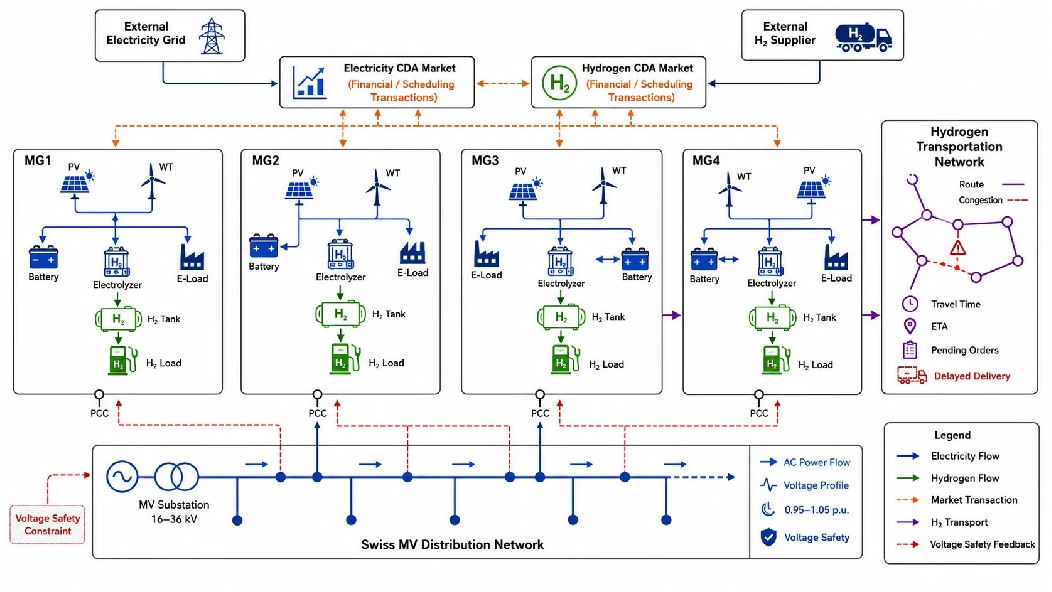
\includegraphics[width=0.96\textwidth]{fig_environment.pdf}
  \caption{电--氢耦合多微电网环境。电力和氢气连续双向拍卖（CDA）决定财务与调度交易；实体氢气经由拥堵交通网络交付；每个微电网通过公共连接点（PCC）接入瑞士中压馈线。}
  \label{fig:environment}
\end{figure*}

\subsection{约束Markov博弈}

系统被建模为包含四个智能体的协作式约束Markov博弈。在时刻$t$，联合状态为$s_t$，智能体$i$接收本地观测$o_t^i$并选择连续动作$a_t^i$。因子化联合策略为
\begin{equation}
  \boldsymbol{\pi}_{\boldsymbol{\theta}}(\boldsymbol{a}_t\mid\boldsymbol{o}_t)
  = \prod_{i=1}^{N}\pi_{\theta_i}(a_t^i\mid o_t^i,h_t^i),
  \qquad N=4,
\end{equation}
其中，$h_t^i$为智能体$i$的GRU Actor隐藏状态。优化目标是最大化日经济期望收益
\begin{equation}
  \label{eq:daily_reward}
  J_R(\boldsymbol{\theta}) = \mathbb{E}_{\boldsymbol{\pi}_{\boldsymbol{\theta}}}
  \left[\sum_{t=0}^{T-1} r_t\right], \qquad T=24,
\end{equation}
并满足全局电压成本约束
\begin{equation}
  J_C(\boldsymbol{\theta}) = \mathbb{E}_{\boldsymbol{\pi}_{\boldsymbol{\theta}}}
  \left[\sum_{t=0}^{T-1} c_t\right] \leq d.
\end{equation}

环境返回原始电压成本$c_t^{\mathrm{raw}}$，Critic目标被归一化为
\begin{equation}
  \label{eq:normalized_cost}
  c_t = \frac{c_t^{\mathrm{raw}}}{0.02}, \qquad d=1.0,
\end{equation}

\subsection{微电网设备、观测与动作}

每个微电网均配置光伏（PV）、风机（WT）、储能电池、电解槽、储氢罐、电负荷和氢负荷。表~\ref{tab:assets}列出了实验中四个异构微电网的设备容量。

\begin{table*}[t]
\centering
\caption{四个微电网智能体的设备容量。电池能量单位为kWh，储氢罐容量单位为kg，储氢充放功率采用低位热值对应的等效能量单位。}
\label{tab:assets}
\small
\begin{tabular}{lrrrrrrr}
\toprule
智能体 & PV (kW) & WT (kW) & 电池 (kWh) & 电池功率 (kW) & 电解槽 (kW) & 储氢罐 (kg) & 储氢功率 (kW$_{\mathrm{H2}}$)\\
\midrule
MG1 & 5000 & 1000 & 5000 & 2000 & 2000 & 500 & 2000\\
MG2 & 1000 & 4000 & 3000 & 1200 & 3000 & 500 & 2000\\
MG3 &  500 & 3000 & 4000 & 1500 &  500 & 300 & 1200\\
MG4 & 2000 &  500 & 2000 &  800 &  800 & 300 & 1500\\
\bottomrule
\end{tabular}
\end{table*}

本地基础观测包含32个归一化特征，用于描述可再生能源出力和负荷、电池荷电状态、氢气库存、近期市场价格与交换功率、时间编码、待到达量分桶、储氢罐剩余容量、线路状况以及本地氢气供应信息。将智能体上一时刻的七维动作拼接后，Actor输入维度为39。分散执行阶段不向智能体提供跨智能体的即时交易广播信息。

动作向量为
\begin{equation}
 a_t^i=[a_{\mathrm{el}},a_{\mathrm{bat}},a_{\mathrm{e,bid}},a_{\mathrm{h,bid}},
 a_{\mathrm{tank}},a_{\mathrm{h,buy}},a_{\mathrm{route}}]^{\top}.
\end{equation}
各分量分别控制电解槽功率、带符号电池功率、电力报价、氢气报价、带符号储氢罐功率、远期购氢量以及线路选择。

\subsection{电力与氢气市场}

电力订单根据实际净电力需求生成，并通过连续双向拍卖完成清算；剩余电力缺额或盈余由外部电网平衡。氢气订单通过类似市场完成清算。当存在交付延迟时，内部CDA撮合成功的氢气在清算时完成财务记录，其实体数量则依据所选线路进入待交付队列。未被内部卖单满足的购氢委托形成经运输交付的常规外购订单，同样经过线路运输后才能进入储氢罐；若当期实际可用氢气仍不足以满足负荷，环境再通过应急购氢即时弥补缺口。常规外购与应急购氢分别对应跨时段补给和当期平衡，二者不重复计量。

运输模块包含四个微电网节点和一个外部供应商节点。每次运输可从三条候选线路中选择一条。可复现的背景交通流具有早晚高峰，线路ETA由有界的美国公路局（BPR）拥堵模型计算。本文评估配置下的ETA约为4--10 h，并计及在途损耗。回合结束前尚未进入本地储氢罐的氢气，其终端资产价值记为零。

\subsection{物理状态转移与能量平衡}
\label{sec:physical_transitions}

环境保留连接不同时刻市场决策的物理状态。令$\Delta t$表示一小时步长，并定义$P_{i,t}^{\mathrm{bat},+}=\max(P_{i,t}^{\mathrm{bat}},0)$和$P_{i,t}^{\mathrm{bat},-}=\max(-P_{i,t}^{\mathrm{bat}},0)$。电池荷电状态更新为
\begin{equation}
  \label{eq:soc_transition}
  \begin{aligned}
  \mathrm{SOC}_{i,t+1}=\operatorname{clip}\!\bigg(&\mathrm{SOC}_{i,t}+
  \frac{\eta_{i,c}^{\mathrm{bat}}P_{i,t}^{\mathrm{bat},+}-P_{i,t}^{\mathrm{bat},-}/\eta_{i,d}^{\mathrm{bat}}}{E_i^{\mathrm{bat},\max}}\Delta t,\\[-1mm]
  &\mathrm{SOC}_i^{\min},\mathrm{SOC}_i^{\max}\bigg).
  \end{aligned}
\end{equation}
动作相关的功率限值在该更新之前施加，从而保证SOC始终位于物理允许范围内。电解槽功率按照下式转换为氢能：
\begin{equation}
  \label{eq:electrolyzer_transition}
  E_{i,t}^{\mathrm{H2,prod}}=\eta_i^{\mathrm{el}}P_{i,t}^{\mathrm{el}}\Delta t,
  \qquad
  E_{i,t}^{\mathrm{H2,load}}=\frac{\sigma_i L_{i,t}^{\mathrm{H}}\Delta t}{\eta^{\mathrm{boiler}}},
\end{equation}
其中，$\sigma_i$为热负荷中由氢气承担的比例。储氢罐功率为正表示充氢，为负表示放氢。类似地定义$P_{i,t}^{\mathrm{tank},+}$和$P_{i,t}^{\mathrm{tank},-}$，则以kg计的储氢量满足
\begin{equation}
  \label{eq:h2_tank_transition}
  H_{i,t+1}=\operatorname{clip}\!\left(H_{i,t}+
  \frac{\eta_{i,c}^{\mathrm{H2}}P_{i,t}^{\mathrm{tank},+}-P_{i,t}^{\mathrm{tank},-}/\eta_{i,d}^{\mathrm{H2}}}{\mathrm{LHV}_{\mathrm{H2}}}\Delta t,\,
  H_i^{\min},H_i^{\max}\right).
\end{equation}

对于每笔撮合成功的氢气交易，交付量首先扣除线路损耗，随后依据ETA进入待到达队列。若$q_{i,t}(\ell)$表示将在$\ell$小时后送达微电网$i$的氢能，则队列可概念性地表示为
\begin{equation}
  \label{eq:pending_transition}
  \begin{aligned}
  q_{i,t+1}(\ell-1)&=q_{i,t}(\ell),\quad \ell\geq1,\\[-1mm]
  q_{i,t+1}(\mathrm{ETA}_{ij,t})&\mathrel{+}=(1-\xi_{ij,t})q_{ij,t}^{\mathrm{clear}}.
  \end{aligned}
\end{equation}
其中，$\xi_{ij,t}$为线路相关损耗率。$\ell=0$时到达的氢气在下一次储氢功率裁剪前加入接收方储氢罐。因此，一笔交易在当前小时完成财务结算，但其实体氢气仅在实际到达时才可用。

传递至两个CDA的本地净平衡量为
\begin{align}
  P_{i,t}^{\mathrm{net,e}} &= L_{i,t}^{\mathrm{e}}+P_{i,t}^{\mathrm{el}}+P_{i,t}^{\mathrm{bat},+}-P_{i,t}^{\mathrm{PV}}-P_{i,t}^{\mathrm{WT}}-P_{i,t}^{\mathrm{bat},-},\label{eq:electric_balance}\\
  E_{i,t}^{\mathrm{net,H2}} &= E_{i,t}^{\mathrm{H2,load}}+P_{i,t}^{\mathrm{tank}}\Delta t-E_{i,t}^{\mathrm{H2,prod}}.\label{eq:h2_balance}
\end{align}
净值为正表示需要购买，为负表示存在可供出售的盈余。CDA首先清算内部订单，剩余量再由相应外部市场平衡。上述状态转移显式刻画了延迟物流状态，而无需引入一般化的Markov状态转移矩阵。

\subsection{配电网潮流与安全成本}

本文选用Swiss-PDGs中的347\_1网络，PCC母线编号为[168, 147, 160, 183]，采用原生20-kV中压网络数据和100-MVA基准容量\cite{swisspdgs}。在每个环境步，将各微电网PCC处的有功、无功注入叠加到网络算例中，并利用兼容MATPOWER的模型通过Newton--Raphson法求解交流潮流\cite{zimmerman2011matpower}。对于母线电压$V_{n,t}$，原始电压成本定义为
\begin{equation}
 c_t^{\mathrm{raw}}=\sum_{n}\left[\max(0,0.95-V_{n,t})
 +\max(0,V_{n,t}-1.05)\right].
\end{equation}
若潮流不收敛，则成本记为1.0。本文所约束的量为系统级电压成本。

\section{所提SGR--MACPO方法}
\label{sec:method}

第~\ref{sec:problem}节中的问题同时包含连续市场动作、非线性交流网络响应、延迟状态转移和分散式观测。集中式在线优化器需要获取各微电网在实际执行阶段无法得到的全局信息，而无约束MARL更新又不能直接控制式~\eqref{eq:normalized_cost}中的电压成本。因此，本文采用集中式训练、分散式循环执行范式，并将约束策略优化改造为适用于单一共享系统安全成本的形式。循环结构用于处理延迟效应和部分可观测后果，独立成本Critic用于估计网络风险，信赖域恢复和接受检验则用于在采样轨迹不可行时限制策略变化。

\subsection{集中式训练与循环Actor}

执行策略采用分散式结构。智能体$i$仅接收$o_t^i$、上一时刻动作及自身循环隐藏状态。GRU对近期控制、库存和交付信息进行汇总，因为这些信息无法从单个瞬时观测中完整推断。在训练阶段，四个本地观测被拼接后输入集中式收益Critic $V_R$和集中式电压成本Critic $V_C$，使两个Critic均能评估各局部动作的联合影响。对于逐小时密集收益轨迹和归一化电压成本轨迹，分别使用广义优势估计；具体参数见表~\ref{tab:training_parameters}。

\subsection{收益与成本代理目标}

令$\hat A_R$和$\hat A_C$分别表示收益优势与成本优势。对于候选Actor参数$\theta$，一阶回合累加代理目标为
\begin{equation}
 L_X(\theta)=\mathbb{E}_{\mathrm{env}}\left[
 \sum_{t=0}^{T-1}\sum_{i=1}^{N}
 \left(\rho_t^i(\theta)-1\right)\hat A_X(t)\right],
 \quad X\in\{R,C\},
\end{equation}
其中，$\rho_t^i$为动作概率比。采样成本估计为
\begin{equation}
 \widetilde J_C(\theta)=\bar C+L_C(\theta).
\end{equation}
之所以采用回合累加形式，是因为若对时间和智能体维度取均值，在当前配置下会将日成本响应缩小约$TN=96$倍。

\subsection{信赖域几何}

该方法计算收益梯度$g_R$、成本梯度$g_C$以及平均KL散度的Hessian矩阵。Fisher向量积通过下式隐式计算：
\begin{equation}
  \label{eq:fisher_vector_product}
  Fv = H_{\mathrm{KL}}v+\eta v,
\end{equation}
其中，$\eta$为阻尼系数。采用共轭梯度近似求解$F^{-1}g_R$和$F^{-1}g_C$。当采样轨迹超过成本预算时，\method 进入保守恢复分支并选择降低成本的方向；当轨迹可行时，若线性化成本不会越过预算，则采用收益方向，否则在成本线性边界与KL椭球的交集上构造更新方向。仅当候选参数通过回溯检验并满足KL上限及对应的收益、成本条件时，才接受该候选参数。该过程将电压约束直接嵌入Actor更新，而无需预先选择固定的收益--成本标量权重。具体更新参数见表~\ref{tab:training_parameters}。

\subsection{可行方向与恢复方向}
\label{sec:update_directions}

令$\Delta\boldsymbol{\theta}$表示拼接后全部Actor参数的同步更新，令$c_0=\widetilde J_C(\boldsymbol{\theta})-d$为采样成本间隙，则局部约束问题为
\begin{equation}
  \label{eq:local_constrained_update}
  \max_{\Delta\boldsymbol{\theta}}\; g_R^{\top}\Delta\boldsymbol{\theta}
  \quad\mathrm{s.t.}\quad c_0+g_C^{\top}\Delta\boldsymbol{\theta}\leq0,\qquad
  \frac{1}{2}\Delta\boldsymbol{\theta}^{\top}F\Delta\boldsymbol{\theta}\leq\delta.
\end{equation}
两个自然梯度坐标分别为$u_R=F^{-1}g_R$和$u_C=F^{-1}g_C$，利用式~\eqref{eq:fisher_vector_product}中的Fisher向量积通过共轭梯度求得。定义
\begin{equation}
  q_R=g_R^{\top}u_R,\qquad q_C=g_C^{\top}u_C,\qquad q_{RC}=g_R^{\top}u_C.
\end{equation}
若$c_0>0$且$q_C>0$，则采样轨迹沿成本恢复方向更新：
\begin{equation}
  \label{eq:recovery_direction}
  \Delta\boldsymbol{\theta}_{\mathrm{rec}}=-\sqrt{\frac{2\delta}{q_C}}\,u_C.
\end{equation}
对于可行轨迹，无约束收益方向为$\Delta\boldsymbol{\theta}_R=\sqrt{2\delta/q_R}\,u_R$。若$c_0+g_C^{\top}\Delta\boldsymbol{\theta}_R\leq0$，则保留该方向；否则将更新置于线性化成本边界和KL椭球的交集上。令
\begin{equation}
  r_\delta=2\delta-\frac{c_0^2}{q_C},\qquad
  q_\perp=q_R-\frac{q_{RC}^2}{q_C},
\end{equation}
则约束方向为
\begin{equation}
  \label{eq:intersection_direction}
  \Delta\boldsymbol{\theta}_{\mathrm{con}}=\alpha u_R+\beta u_C,\qquad
  \alpha=\sqrt{\frac{r_\delta}{q_\perp}},\qquad
  \beta=\frac{-c_0-\alpha q_{RC}}{q_C},
\end{equation}
前提是各分母和剩余KL半径均为正。上述公式描述了面向共享系统的具体实现：四个循环Actor利用同一个电压成本梯度共同更新，而非采用其他多智能体安全策略方法中的逐智能体顺序分解。

\subsection{基于采样成本的回溯线搜索}
\label{sec:backtracking}

对于选定方向$\Delta\boldsymbol{\theta}$，候选参数生成方式为
\begin{equation}
  \label{eq:backtracking_candidate}
  \boldsymbol{\theta}^{(k)}=\boldsymbol{\theta}+\zeta^k\Delta\boldsymbol{\theta},\qquad
  k=0,\ldots,K-1,
\end{equation}
其中，本文实验设置$\zeta=0.5$、$K=10$。每个候选参数均通过采样收益代理目标、采样电压成本目标和平均KL散度进行评估。当恢复候选的采样成本不高于当前采样成本且KL散度不超过$\delta$时接受该候选；收益候选或约束收益候选还必须同时满足采样成本预算且不降低采样收益。第一个满足这些条件的候选参数将被应用。该显式接受步骤避免将线性化代理目标作为唯一的安全检验。

最终更新流程为：采集循环轨迹；拟合集中的收益Critic和电压成本Critic；分别计算两类优势与梯度；求解隐式Fisher方程；选择收益、约束收益或恢复方向；应用基于采样成本的回溯线搜索。图~\ref{fig:algorithm}给出了该流程的简要示意。

\begin{figure}[t]
  \centering
  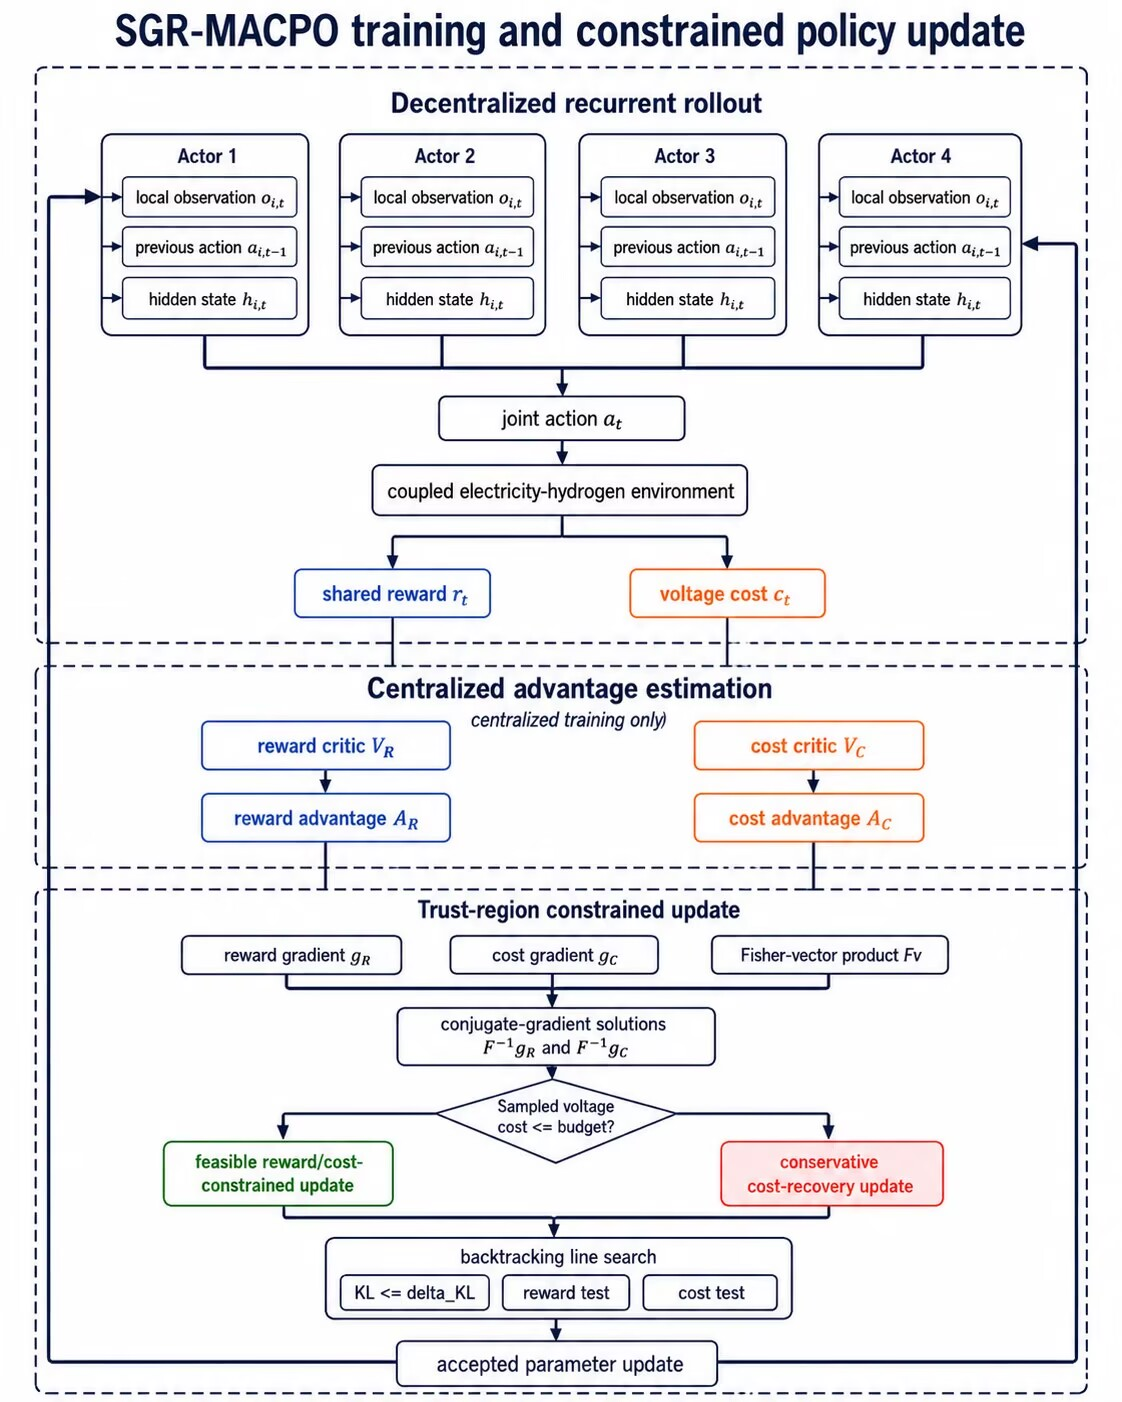
\includegraphics[width=0.98\columnwidth]{fig_algorithm_image2.png}
  \caption{\method 的训练与约束策略更新流程。分散式循环Actor与耦合环境交互，收益Critic和电压成本Critic仅在训练阶段集中使用；可行更新和恢复更新在回溯过程中接受KL、收益和成本检验。}
  \label{fig:algorithm}
\end{figure}

\section{算例与结果分析}
\label{sec:experiments}

\subsection{评估方案与指标}

主要运行性能对比采用三个可复现的确定性测试日与交通流场景。对比方法包括无约束MAPPO、固定罚项MAPPO和\method；三者使用相同的环境、观测与动作空间以及GRU Actor--Critic架构，主要区别在于策略更新方式。Lagrangian控制器仅用于训练曲线诊断，不纳入三日运行结果表。

算例围绕本文贡献回答四个问题：（i）约束感知更新能否改善电压安全与经济性的平衡；（ii）电力CDA清算如何经由剩余电网交换传导至电压轨迹；（iii）氢气CDA与常规外购订单如何通过延迟交付影响闭环运行；（iv）循环Actor是否实际利用时序输入。经济性能以累计运行成本（百万元人民币）表示，网络性能采用原始电压成本、最低母线电压和逐小时越限曲线表示。

表~\ref{tab:training_parameters}汇总了主要训练和更新参数，其中$\gamma=1$与24 h不折扣调度目标一致，\method 的Actor采用约束自然梯度更新。

\begin{table}[t]
\centering
\caption{Env-v6对比实验所采用的训练及更新参数，并明确列出各方法专属设置。}
\label{tab:training_parameters}
\scriptsize
\setlength{\tabcolsep}{4.0pt}
\begin{tabular}{ll}
\toprule
设置 & 数值\\
\midrule
GRU隐藏层维度（Actor/Critic） & 128\\
Actor输入维度 & 39\\
并行环境数$\times$时域长度 & $2\times24$\\
训练更新次数 & 1000\\
折扣因子$\gamma$ / GAE参数$\lambda$ & 1.0 / 0.95\\
Adam学习率 & $3\times10^{-4}\!\rightarrow0$\\
MAPPO裁剪参数 / 熵系数 & 0.2 / 0.01\\
罚项MAPPO成本系数$\alpha$ & 1.0\\
SGR--MACPO原始/归一化预算 & 0.02 / 1.0\\
SGR--MACPO的KL / CG / 阻尼 & 0.01 / 10 / $10^{-2}$\\
SGR--MACPO回溯次数 / 比例 & 10 / 0.5\\
\bottomrule
\end{tabular}
\end{table}

\begin{table}[t]
\centering
\caption{各方法基于单个训练策略的三日确定性Env-v6测试结果。所有控制器均采用GRU策略。}
\label{tab:main_results}
\scriptsize
\setlength{\tabcolsep}{3.2pt}
\begin{tabular}{lcc}
\toprule
方法 & 电压成本 & 成本（百万元）\\
\midrule
MAPPO & 7.757 & 2.94\\
固定罚项MAPPO & 1.409 & 23.53\\
\method & 0.685 & 11.90\\
\bottomrule
\end{tabular}
\end{table}

\begin{figure}[t]
  \centering
  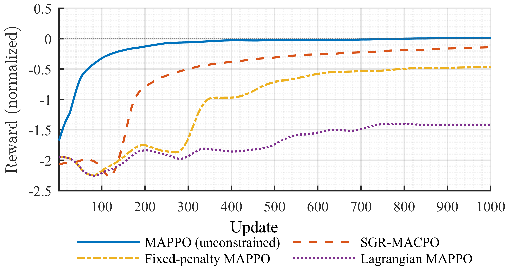
\includegraphics[width=0.98\columnwidth]{fig_convergence_reward.pdf}
  \caption{各对比算法的缩放训练收益轨迹。为使单栏图中的安全--经济权衡更清晰，收益曲线与电压成本曲线分别绘制。}
  \label{fig:reward_convergence}
\end{figure}

\begin{figure}[t]
  \centering
  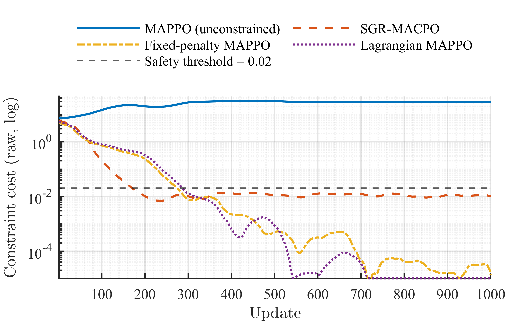
\includegraphics[width=0.98\columnwidth]{fig_convergence_voltage_cost.pdf}
  \caption{对数坐标下的原始训练电压成本轨迹。水平虚线表示0.02的原始日电压成本预算。}
  \label{fig:cost_convergence}
\end{figure}

\FloatBarrier
\subsection{总体性能}
\label{sec:results}

表~\ref{tab:main_results}中，无约束MAPPO取得最低经济成本，但其电压越限最严重。固定罚项MAPPO能够减少越限，却付出了显著更高的经济成本，说明固定收益--成本权重具有较强敏感性。与MAPPO和固定罚项MAPPO相比，\method 的三日累计原始电压成本分别降低91.2\%和51.4\%，同时其经济成本低于后者。

图~\ref{fig:reward_convergence}和图~\ref{fig:cost_convergence}分别展示经济目标与安全目标的收敛过程。无约束MAPPO获得最高收益，但始终高于电压成本预算；\method 收敛至相对较低的收益，同时有效降低成本信号；固定罚项和Lagrangian更新虽然也能获得较低电压成本，却带来更大的经济损失。因此，该结果反映的是安全性与经济性的权衡，而非单纯的收益优势。

\subsection{电力CDA驱动的网络安全算例}
\label{sec:cda_network_case}

CDA是连接分散式动作与网络安全成本的关键环节。在每个小时，Actor首先决定本地设备运行，由此形成实际净电力需求和净氢气需求，同时给出对应的报价与数量。随后，电力CDA按照价格--时间优先原则撮合内部卖方与买方，只有未被内部交易覆盖的剩余缺额或盈余才与外部电网结算。氢气CDA采用相同的市场逻辑，但成交氢气在财务上即时清算，其实体数量则依据线路相关ETA进入交付队列。

\begin{figure}[t]
  \centering
  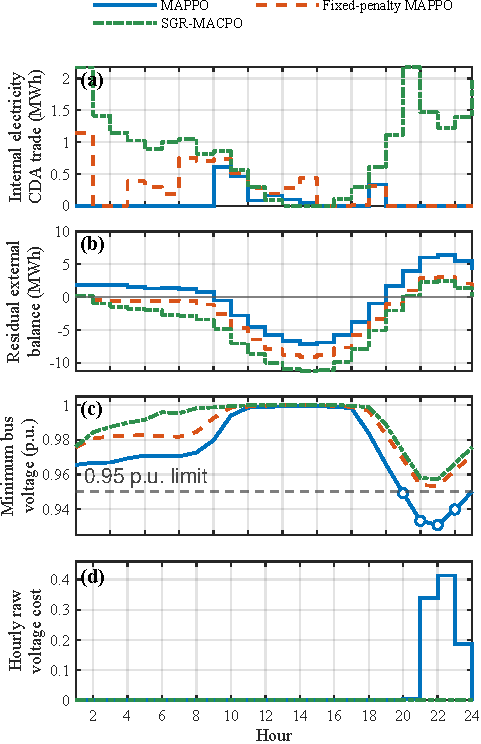
\includegraphics[width=0.98\columnwidth]{fig_voltage_case_seed32.pdf}
  \caption{代表性场景下从电力CDA到配电网的作用链：（a）内部CDA成交量；（b）清算后的外部剩余平衡量（正值表示购电）；（c）馈线最低母线电压；（d）原始电压成本。空心圆标记MAPPO的低电压时段。}
  \label{fig:voltage_case}
\end{figure}

图~\ref{fig:voltage_case}展示了代表性场景下的“市场--网络”作用链。全天内，\method 的内部电力CDA成交量为21.66~MWh，而MAPPO和固定罚项MAPPO分别仅为1.80~MWh和6.24~MWh。在20--24 h关键时段，\method 通过内部市场成交8.22~MWh，使外部购电残差仅为6.44~MWh；两种基线在此期间均无内部电力成交，外部购电分别达到26.21~MWh和15.82~MWh。相应地，MAPPO在20--23 h低于0.95~p.u.，最低降至0.9309~p.u.，累计原始电压成本为0.943。固定罚项MAPPO和\method 均保持在电压下限以上，最低电压分别为0.9533和0.9572~p.u.，电压成本均为0。由于三种方法采用相同的CDA规则、环境、循环网络架构、观测与动作空间，因此上述内部清算与剩余平衡差异来自不同策略更新所学习到的运行方式。\method 中独立的系统电压成本方向，使策略能够在晚高峰主动利用内部协调，同时将剩余PCC交换维持在电压安全轨迹上。

四个子图还呈现出三个具有明确物理含义的运行阶段。1--8 h期间，\method 的内部CDA成交量保持在0.82--2.17~MWh，而两种基线大多只有少量或没有内部电力成交；因此，其外部剩余交换由少量购电逐步转为适度售电，而不是持续依赖外部购电。9--18 h期间，随着本地发电超过聚合负荷，三种方法的外部剩余平衡均转为负值；与此同时，约13--15 h的内部成交量趋近于零，说明此时订单簿中的买卖报价与数量缺乏足够重叠，剩余电力因而直接向外部电网出售。19 h以后，方法间再次出现显著分离：MAPPO的外部购电由1.72~MWh增至6.46~MWh，最低电压由0.9659~p.u.降至0.9309~p.u.；固定罚项MAPPO在22 h将购电限制至3.10~MWh；\method 则在19--24 h保持1.11--2.18~MWh的内部CDA成交量，并将外部购电控制在2.45~MWh以下。这种按时段对应的差异正是系统级电压成本方向在运行层面的表现：策略在剩余不平衡到达PCC之前，首先改变各微电网盈余服务本地缺额的方式。正如含网络约束的P2P安全分析所强调的\cite{ma2025network}，能够体现贡献的证据不仅是最终电压数值，还包括电压变化之前发生的交易模式改变。

\subsection{氢气CDA与交付时序反事实实验}

\begin{figure}[t]
  \centering
  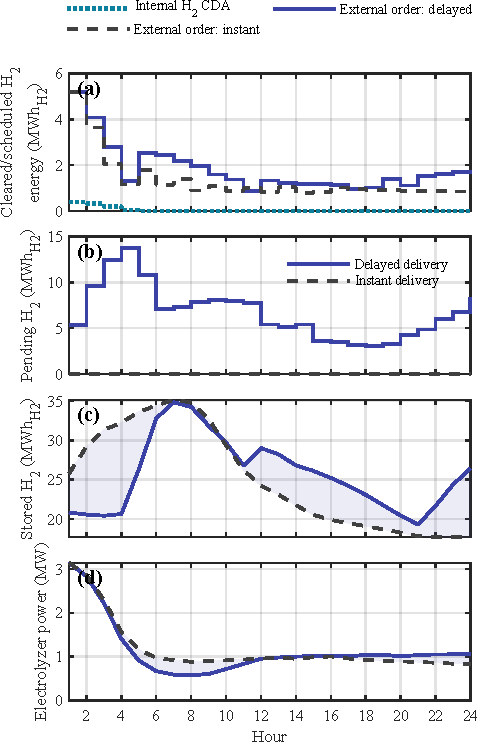
\includegraphics[width=0.98\columnwidth]{fig_h2_delay_case_seed32_singlecol.pdf}
  \caption{代表性场景下延迟交付与即时交付两种情形的“氢气市场--物流交付”作用链：（a）内部氢气CDA成交量及常规外购订单；（b）在途待交付氢能；（c）储存氢能；（d）电解槽功率。实验仅改变实体交付时序，策略检查点和观测维度保持不变。}
  \label{fig:h2_delay_case}
\end{figure}

为隔离交付时序影响，本文采用同一个\method 策略检查点，分别在拥堵相关延迟交付和即时交付条件下进行闭环评估，且不重新训练策略参数。每小时内部氢气CDA首先清算买卖订单，未被内部卖单满足的购氢委托形成常规外购订单；延迟场景中，这两类成交量均经过运输队列交付，反事实场景中则即时到达。两条轨迹的内部氢气CDA成交量均为0.96~MWh$_{\mathrm{H2}}$，而延迟交付使常规外购订单由31.8增至43.4~MWh$_{\mathrm{H2}}$。交付延迟由此形成持续的在途库存，并进一步改变储氢量和电解槽运行：5--10 h的电解槽功率低于即时交付场景，而19--24 h则更高。两种情形的应急氢气供应量分别为43.2和32.1~MWh$_{\mathrm{H2}}$；在延迟场景的回合终点，仍有8.38~MWh$_{\mathrm{H2}}$处于待交付状态，而即时交付场景为零。

图~\ref{fig:h2_delay_case}中各曲线升降方向均具有明确物理含义。1--4 h期间，延迟场景的在途氢能逐步累积至13.78~MWh$_{\mathrm{H2}}$，即时交付场景则不存在运输队列。当前期货运开始到达并暂时补充储氢罐后，延迟场景控制器在5--10 h将电解槽功率降低至即时交付轨迹以下。12--20 h期间，延迟场景的在途库存由5.41降至3.05~MWh$_{\mathrm{H2}}$，储氢量由29.0降至20.4~MWh$_{\mathrm{H2}}$，同时电解槽功率回升至约1.04~MW。21--24 h期间，延迟运输队列再次增至8.38~MWh$_{\mathrm{H2}}$，储氢量回升至26.4~MWh$_{\mathrm{H2}}$，电解槽功率相应维持在约1.04--1.06~MW；相比之下，即时交付轨迹的电解槽功率降至0.83~MW，储氢量稳定在约17.7~MWh$_{\mathrm{H2}}$。延迟使常规外购订单增加36.5\%，反映了订单到达滞后、库存变化以及后续CDA和外购决策之间的闭环反馈。

\subsection{循环信息消融实验}
\label{sec:recurrent_ablation}

为明确体现循环策略输入的贡献，本文进行两组基于同一检查点、同一测试日的实验，每次只移除一种时序输入。图~\ref{fig:recurrent_ablation}给出了相应经济成本。与完整控制器相比，移除GRU隐藏状态后成本增加56.5\%，移除上一时刻动作后成本增加127.8\%。这种有序的性能退化说明，在协调储能、氢气交付和网络运行时，策略同时利用了累积历史和紧邻的上一时刻控制信号；其中，上一动作通道对维持短时域控制连续性尤为重要。

\begin{figure}[t]
  \centering
  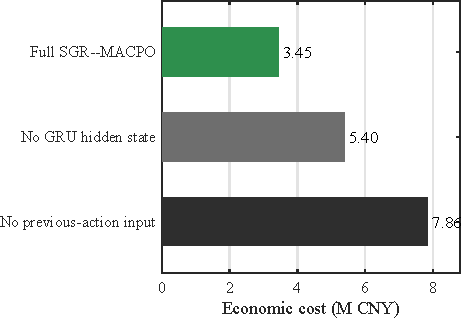
\includegraphics[width=0.98\columnwidth]{fig_recurrent_ablation_seed30.pdf}
  \caption{代表性测试场景下基于同一检查点的循环信息消融实验。每次只移除图示时序输入，其余策略参数和物理设置保持不变。}
  \label{fig:recurrent_ablation}
\end{figure}

\FloatBarrier
\section{讨论}
\label{sec:discussion}

上述结果将各项方法设计与可观测的运行效果建立了对应关系。独立的电压成本方向与回溯检验使电力CDA形成相应的内部清算模式和外部剩余平衡轨迹，从而在维持晚高峰内部协调的同时避免低电压事件。在氢能链条中，内部CDA成交量和常规外购订单共同形成在途库存；显式交付时序随后改变库存，并在策略检查点保持不变时继续反馈至后续订单、储氢和电解槽运行。循环信息消融还表明，累积历史与上一时刻动作均有助于实现经济的闭环运行。综合来看，实验从市场、网络和多能源运行三个层面，将策略更新设计、双市场清算、延迟物理状态和循环执行架构与实际运行效果联系起来。

\section{结论}
\label{sec:conclusion}

本文提出了面向电--氢耦合多微电网循环多智能体调度的\method。该方法结合分散式GRU Actor、集中式收益与电压成本Critic，以及包含显式恢复方向和采样成本回溯检验的共享系统信赖域更新。在Env-v6对比实验中，\method 相较无约束MAPPO显著减少电压越限，并比固定罚项MAPPO获得更有利的经济性权衡。运行算例进一步追踪了电力CDA清算至剩余网络交换的传导过程，以及氢气CDA和常规外购订单经过延迟交付队列影响储氢与转换设备的过程。移除循环状态或上一动作信息均会显著增加经济成本。

\section*{数据可用性}

本文使用的Swiss-PDGs配电网数据公开发布于\url{https://github.com/aeonetos/Swiss-PDGs}。支撑本文结果的环境配置、训练检查点和处理后评估数据将在开放研究仓库中发布，永久仓库链接将在投稿前补充。在此之前，处理后的数据可根据合理请求向通信作者获取。

\begin{thebibliography}{00}

\bibitem{yue2021hydrogen}
M. Yue, H. Lambert, E. Pahon, R. Roche, S. Jemei, D. Hissel, Hydrogen energy systems: A critical review of technologies, applications, trends and challenges, Renewable and Sustainable Energy Reviews 146 (2021) 111180. \url{https://doi.org/10.1016/j.rser.2021.111180}.

\bibitem{li2023hierarchical}
Q. Li, X. Xiao, Y. Pu, S. Luo, H. Liu, W. Chen, Hierarchical optimal scheduling method for regional integrated energy systems considering electricity-hydrogen shared energy, Applied Energy 349 (2023) 121670. \url{https://doi.org/10.1016/j.apenergy.2023.121670}.

\bibitem{he2025hydrogen}
W. He, C. Cai, Q.-L. Han, X. Qing, W. Du, F. Qian, Optimal scheduling of a hydrogen-based microgrid for an industrial park: A reinforcement learning approach, IEEE Transactions on Systems, Man, and Cybernetics: Systems 55 (6) (2025) 4348--4361. \url{https://doi.org/10.1109/TSMC.2025.3551325}.

\bibitem{paudel2019p2p}
A. Paudel, K. Chaudhari, C. Long, H.B. Gooi, Peer-to-peer energy trading in a prosumer-based community microgrid: A game-theoretic model, IEEE Transactions on Industrial Electronics 66 (8) (2019) 6087--6097. \url{https://doi.org/10.1109/TIE.2018.2874578}.

\bibitem{samadi2020decentralized}
E. Samadi, A. Badri, R. Ebrahimpour, Decentralized multi-agent based energy management of microgrid using reinforcement learning, International Journal of Electrical Power \& Energy Systems 122 (2020) 106211. \url{https://doi.org/10.1016/j.ijepes.2020.106211}.

\bibitem{fang2021multiagent}
X. Fang, Q. Zhao, J. Wang, Y. Han, Y. Li, Multi-agent deep reinforcement learning for distributed energy management and strategy optimization of microgrid market, Sustainable Cities and Society 74 (2021) 103163. \url{https://doi.org/10.1016/j.scs.2021.103163}.

\bibitem{zhang2023interconnected}
B. Zhang, W. Hu, A.M.Y.M. Ghias, X. Xu, Z. Chen, Multi-agent deep reinforcement learning based distributed control architecture for interconnected multi-energy microgrid energy management and optimization, Energy Conversion and Management 277 (2023) 116647. \url{https://doi.org/10.1016/j.enconman.2022.116647}.

\bibitem{glavic2017reinforcement}
M. Glavic, R. Fonteneau, D. Ernst, Reinforcement learning for electric power system decision and control: Past considerations and perspectives, IFAC-PapersOnLine 50 (1) (2017) 6918--6927. \url{https://doi.org/10.1016/j.ifacol.2017.08.1217}.

\bibitem{cao2020review}
D. Cao, W. Hu, J. Zhao, G. Zhang, B. Zhang, Z. Liu, Reinforcement learning and its applications in modern power and energy systems: A review, Journal of Modern Power Systems and Clean Energy 8 (6) (2020) 1029--1042. \url{https://doi.org/10.35833/MPCE.2020.000552}.

\bibitem{bahrami2021demand}
S. Bahrami, Y.C. Chen, V.W.S. Wong, Deep reinforcement learning for demand response in distribution networks, IEEE Transactions on Smart Grid 12 (2) (2021) 1496--1506. \url{https://doi.org/10.1109/TSG.2020.3037066}.

\bibitem{lowe2017maddpg}
R. Lowe, Y. Wu, A. Tamar, J. Harb, P. Abbeel, I. Mordatch, Multi-agent actor-critic for mixed cooperative-competitive environments, in: Advances in Neural Information Processing Systems 30, 2017, pp. 6379--6390.

\bibitem{foerster2018coma}
J. Foerster, G. Farquhar, T. Afouras, N. Nardelli, S. Whiteson, Counterfactual multi-agent policy gradients, Proceedings of the AAAI Conference on Artificial Intelligence 32 (1) (2018) 2974--2982. \url{https://doi.org/10.1609/aaai.v32i1.11794}.

\bibitem{schulman2017ppo}
J. Schulman, F. Wolski, P. Dhariwal, A. Radford, O. Klimov, Proximal policy optimization algorithms, arXiv:1707.06347, 2017. \url{https://doi.org/10.48550/arXiv.1707.06347}.

\bibitem{yu2022mappo}
C. Yu, A. Velu, E. Vinitsky, J. Gao, Y. Wang, A.M. Bayen, Y. Wu, The surprising effectiveness of PPO in cooperative multi-agent games, in: Advances in Neural Information Processing Systems 35, 2022, pp. 24611--24624. \url{https://doi.org/10.52202/068431-1787}.

\bibitem{gronauer2022survey}
S. Gronauer, K. Diepold, Multi-agent deep reinforcement learning: A survey, Artificial Intelligence Review 55 (2) (2022) 895--943. \url{https://doi.org/10.1007/s10462-021-09996-w}.

\bibitem{achiam2017cpo}
J. Achiam, D. Held, A. Tamar, P. Abbeel, Constrained policy optimization, in: Proceedings of the 34th International Conference on Machine Learning, Proceedings of Machine Learning Research 70, 2017, pp. 22--31.

\bibitem{gu2021macpo}
S. Gu, J.G. Kuba, M. Wen, R. Chen, Z. Wang, Z. Tian, J. Wang, A. Knoll, Y. Yang, Multi-agent constrained policy optimisation, arXiv:2110.02793, 2021. \url{https://doi.org/10.48550/arXiv.2110.02793}.

\bibitem{ma2025network}
Q. Ma, Z. Liu, Y. Ye, X. Liu, Network-constrained P2P trading: A safety-aware decentralized multi-agent reinforcement learning approach, IEEE Transactions on Smart Grid 16 (6) (2025) 5573--5588. \url{https://doi.org/10.1109/TSG.2025.3589888}.

\bibitem{liu2025carbon}
X. Liu, Y. Ye, S. Li, C. Zhang, Q. Ma, J. Zhu, Carbon-aware peer-to-peer energy trading in an unbalanced distribution network via a Nash equilibrium discovery deep reinforcement learning approach, IEEE Transactions on Smart Grid 16 (4) (2025) 3392--3405. \url{https://doi.org/10.1109/TSG.2025.3561515}.

\bibitem{hausknecht2015drqn}
M. Hausknecht, P. Stone, Deep recurrent Q-learning for partially observable MDPs, arXiv:1507.06527, 2015. \url{https://doi.org/10.48550/arXiv.1507.06527}.

\bibitem{vazquez2019demand}
J.R. V\'azquez-Canteli, Z. Nagy, Reinforcement learning for demand response: A review of algorithms and modeling techniques, Applied Energy 235 (2019) 1072--1089. \url{https://doi.org/10.1016/j.apenergy.2018.11.002}.

\bibitem{francois2018deep}
V. Fran\c{c}ois-Lavet, P. Henderson, R. Islam, M.G. Bellemare, J. Pineau, An introduction to deep reinforcement learning, Foundations and Trends in Machine Learning 11 (3--4) (2018) 219--354. \url{https://doi.org/10.1561/2200000071}.

\bibitem{staffell2019hydrogen}
I. Staffell, D. Scamman, A. Velazquez Abad, P. Balcombe, P.E. Dodds, P. Ekins, N. Shah, K.R. Ward, The role of hydrogen and fuel cells in the global energy system, Energy \& Environmental Science 12 (2) (2019) 463--491. \url{https://doi.org/10.1039/C8EE01157E}.

\bibitem{parra2019hydrogen}
D. Parra, L. Valverde, F.J. Pino, M.K. Patel, A review on the role, cost and value of hydrogen energy systems for deep decarbonisation, Renewable and Sustainable Energy Reviews 101 (2019) 279--294. \url{https://doi.org/10.1016/j.rser.2018.11.010}.

\bibitem{glenk2019economics}
G. Glenk, S. Reichelstein, Economics of converting renewable power to hydrogen, Nature Energy 4 (3) (2019) 216--222. \url{https://doi.org/10.1038/s41560-019-0326-1}.

\bibitem{almansoori2009supply}
A. Almansoori, N. Shah, Design and operation of a future hydrogen supply chain: Multi-period model, International Journal of Hydrogen Energy 34 (19) (2009) 7883--7897. \url{https://doi.org/10.1016/j.ijhydene.2009.07.109}.

\bibitem{moreno2017infrastructure}
M. Moreno-Benito, P. Agnolucci, L.G. Papageorgiou, Towards a sustainable hydrogen economy: Optimisation-based framework for hydrogen infrastructure development, Computers \& Chemical Engineering 102 (2017) 110--127. \url{https://doi.org/10.1016/j.compchemeng.2016.08.005}.

\bibitem{tushar2020p2p}
W. Tushar, T.K. Saha, C. Yuen, D. Smith, H.V. Poor, Peer-to-peer trading in electricity networks: An overview, IEEE Transactions on Smart Grid 11 (4) (2020) 3185--3200. \url{https://doi.org/10.1109/TSG.2020.2969657}.

\bibitem{sousa2019p2p}
T. Sousa, T. Soares, P. Pinson, F. Moret, T. Baroche, E. Sorin, Peer-to-peer and community-based markets: A comprehensive review, Renewable and Sustainable Energy Reviews 104 (2019) 367--378. \url{https://doi.org/10.1016/j.rser.2019.01.036}.

\bibitem{morstyn2018p2p}
T. Morstyn, N. Farrell, S.J. Darby, M.D. McCulloch, Using peer-to-peer energy-trading platforms to incentivize prosumers to form federated power plants, Nature Energy 3 (2) (2018) 94--101. \url{https://doi.org/10.1038/s41560-017-0075-y}.

\bibitem{sunehag2018vdn}
P. Sunehag, G. Lever, A. Gruslys, W.M. Czarnecki, V. Zambaldi, M. Jaderberg, M. Lanctot, N. Sonnerat, J.Z. Leibo, K. Tuyls, T. Graepel, Value-decomposition networks for cooperative multi-agent learning based on team reward, in: Proceedings of the 17th International Conference on Autonomous Agents and MultiAgent Systems, 2018, pp. 2085--2087.

\bibitem{rashid2020qmix}
T. Rashid, M. Samvelyan, C. Schroeder de Witt, G. Farquhar, J. Foerster, S. Whiteson, QMIX: Monotonic value function factorisation for deep multi-agent reinforcement learning, in: Proceedings of the 35th International Conference on Machine Learning, Proceedings of Machine Learning Research 80, 2018, pp. 4295--4304. \url{https://doi.org/10.48550/arXiv.1803.11485}.

\bibitem{hernandez2019survey}
P. Hernandez-Leal, B. Kartal, M.E. Taylor, A survey and critique of multiagent deep reinforcement learning, Autonomous Agents and Multi-Agent Systems 33 (6) (2019) 750--797. \url{https://doi.org/10.1007/s10458-019-09421-1}.

\bibitem{oroojlooy2023review}
A. Oroojlooy, D. Hajinezhad, A review of cooperative multi-agent deep reinforcement learning, Applied Intelligence 53 (11) (2023) 13677--13722. \url{https://doi.org/10.1007/s10489-022-04105-y}.

\bibitem{papoudakis2021benchmark}
G. Papoudakis, F. Christianos, L. Sch\"afer, S.V. Albrecht, Benchmarking multi-agent deep reinforcement learning algorithms in cooperative tasks, in: Advances in Neural Information Processing Systems 34, Datasets and Benchmarks Track, 2021. \url{https://doi.org/10.48550/arXiv.2006.07869}.

\bibitem{garcia2015safe}
J. Garc\'ia, F. Fern\'andez, A comprehensive survey on safe reinforcement learning, Journal of Machine Learning Research 16 (42) (2015) 1437--1480.

\bibitem{schulman2015trpo}
J. Schulman, S. Levine, P. Abbeel, M. Jordan, P. Moritz, Trust region policy optimization, in: Proceedings of the 32nd International Conference on Machine Learning, Proceedings of Machine Learning Research 37, 2015, pp. 1889--1897.

\bibitem{chow2018lyapunov}
Y. Chow, O. Nachum, E.A. Du\'e\~nez-Guzm\'an, M. Ghavamzadeh, A Lyapunov-based approach to safe reinforcement learning, in: Advances in Neural Information Processing Systems 31, 2018, pp. 8092--8101. \url{https://doi.org/10.48550/arXiv.1805.07708}.

\bibitem{tessler2019reward}
C. Tessler, D.J. Mankowitz, S. Mannor, Reward constrained policy optimization, in: Proceedings of the 7th International Conference on Learning Representations, 2019. \url{https://doi.org/10.48550/arXiv.1805.11074}.

\bibitem{ray2019benchmark}
A. Ray, J. Achiam, D. Amodei, Benchmarking safe exploration in deep reinforcement learning, arXiv:1910.01708, 2019. \url{https://doi.org/10.48550/arXiv.1910.01708}.

\bibitem{swisspdgs}
A. Eonetos, Swiss-PDGs: Swiss distribution grid data, GitHub repository. \url{https://github.com/aeonetos/Swiss-PDGs} (accessed 23 August 2026).

\bibitem{zimmerman2011matpower}
R.D. Zimmerman, C.E. Murillo-Sanchez, R.J. Thomas, MATPOWER: Steady-state operations, planning, and analysis tools for power systems research and education, IEEE Transactions on Power Systems 26 (1) (2011) 12--19. \url{https://doi.org/10.1109/TPWRS.2010.2051168}.

\end{thebibliography}

\balance

\end{document}
